\documentclass[journal]{IEEEtran}
\usepackage{xcolor}
\usepackage{cite}
\usepackage{amsmath,amssymb,amsfonts}
\usepackage{algorithm}
\usepackage{algpseudocode}
%\usepackage{algorithmic}
\usepackage{graphicx}
\usepackage{textcomp}
\usepackage{graphicx}
%\usepackage{caption}
\usepackage{subcaption}
\usepackage[hyphens]{url}

% correct bad hyphenation here
% \hyphenation{op-tical net-works semi-conduc-tor}

\begin{document}

\title{ELEC1601 Exercise 3 Lab Report}

\author{SID: 520464588 Lab Group: F09 Group 8}

% make the title area
\maketitle


\begin{abstract}
Very briefly: What was the goal of this work? What you did you do to achieve this? What did you learn?
In this lab, the goal was to understand how we could create a maze navigating robot, by experimenting with  continuous servos, light and IR sensors. 
\end{abstract}


\section{Introduction}

\IEEEPARstart{T}{he} purpose of this lab session was to learn how 

… (what you think we want you to learn/skills we want you to develop)

Overview the methods that you used to achieve the learning outcomes you just stated, including software, hardware and teamwork.

State what  you achieved in your final implementation.

\section{Background}
The exercise consisted of using continuous servos, light sensors and IR sensors, along with the Arduino, wires, resistors and a breadboard. Further, the code was structured in an object oriented style in order to maintain readability due to the scale of the project. These components were simulated in TinkerCAD before importing the code to the physical components with the Arduino IDE.
%Overview any related background information. This should include components and tools used in lab (include all components: LEDs, resistors, diodes). For every component that is not minor (e.g. wires), you should discuss briefly what they do/how they work (E.g. under what conditions does an LED produce light, what affects it’s brightness), how you will use them. Furthermore, give examples of real-world uses of these components (e.g. LEDs are increasingly used in lighting rooms, but also indicators for digital devices.

%You can, but do not have to use the following sub-headings:

\subsection{Software}
\begin{itemize}
    \item{Object oriented programming was used to separate functionality between classes for better scalability.}
    \item{TinkerCAD was used to simulate the physical Arduino components to test if the code works as expected.}
    \item{The Arduino IDE was used to check if the code compiles and to load it on to the physical Arduino.}
\end{itemize}
\subsection{Hardware}
\begin{itemize}
    \item{Light sensors write an analog value based on how much light they are exposed to, with higher values indicating stronger intensity.}
    \item{Continuous servos consists of a gear and shaft that can be controlled by the pins on the Arduino, such that the shaft can be rotated by 360 degrees.}
    \item{The Arduino computer was connected to the other physical components. Analog input pins were used to read the output values of the sensors, while the output PWM pins were used to control the rotation of the servos.}
    \item{Wires}
    \item{Resistors}
    \item{Breadboard}
\end{itemize}

%You can, but do not have to use tables. If you do, an example of how you might format one is given in Table ~\ref{tab1}, which describes a summary of all the materials required for this laboratory exercise.

\newpage
\begin{table}[htbp]
\caption{Summary of all components. (You can, but do not have to include this table. This table example is an example of how to add a table to  your document, and how to construct in Latex)}
\begin{center}
\begin{tabular}{|c|c|c|}
\hline
\textbf{Component} & \textbf{\textit{Number required}}& \textbf{\textit{Other details}}\\
\hline
LED& 4 &  \\
Resistor& 10 &  330 Ohm\\
\hline
\end{tabular}
\label{tab1}
\end{center}
\end{table}

\section{Method}

%For each part of the lab, describe the circuit you created, and describe your code with pseudocode. Explain what this pseudocode does and how it interacts with your circuit drawing using text in this section. Explain any design decisions made (why use LED/how you chose your values to send from Arduino to the LED, why you chose a given resistor size if important). Discuss any limitations/successes/unexpected results.

% Highlight how you built on aspects you created in earlier parts of the lab where possible).

% Describe any differences/challenges in moving from software to hardware..

% Use Figures/Tables/Algorithms as appropriate.

\subsection{Part I}
For the virtual component of Part 1, we simulated the the use of a light sensor and reading it's analog input from the Arduino board. The sensor was connected to the 5V power source, along with a 10K Ohm resistor to GND. The output was read using an analog input pin, namely A0. In order to account for scalability, the code was structured using the object-oriented paradigm, with the UML class diagram for the LightSensor class used in this part depicted in Figure~\ref{fig:uml1}. 
The algorithm connecting the code to the desired functionality described above is referenced in Algorithm~\ref{alg:part1algo} and describes initialising a LightSensor object and printing it's output to the terminal. It was observed that as the light intensity increased, the analog output value also increased.
%(Example text of how to cite/how to reference tables). In Part 1, we emulated the circuit described in the lab instructions \cite{elec1601_notes} (this is how we write a reference). Another example is the book by Harris and Harris~\cite{harris2010digital}. Algorithm~\ref{alg:part1} (Example how to reference an algorithm). Describes our program to make this circuit run. (Please note, pseudocode is code that describes the algorithm in such a fashion it can be easily translated into any programming language. It should not have any specific syntax e.g. C/JAVA/Python)
\begin{figure}[ht]
    \centering
      \begin{subfigure}[b]{0.2\textwidth}
         \centering
         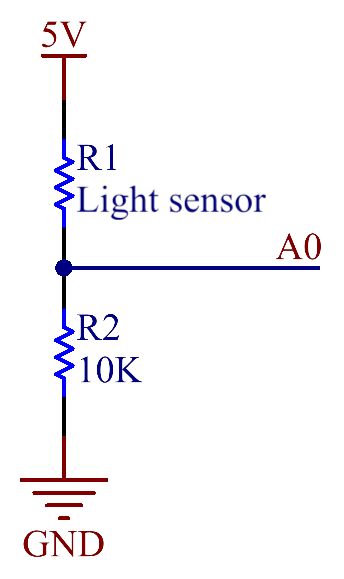
\includegraphics[width=0.2\textwidth]{images/pt1.png} 
         \caption{Circuit Diagram}
         \label{fig:Circuit_diagram1}
     \end{subfigure}
     \begin{subfigure}[b]{0.2\textwidth}
         \centering
         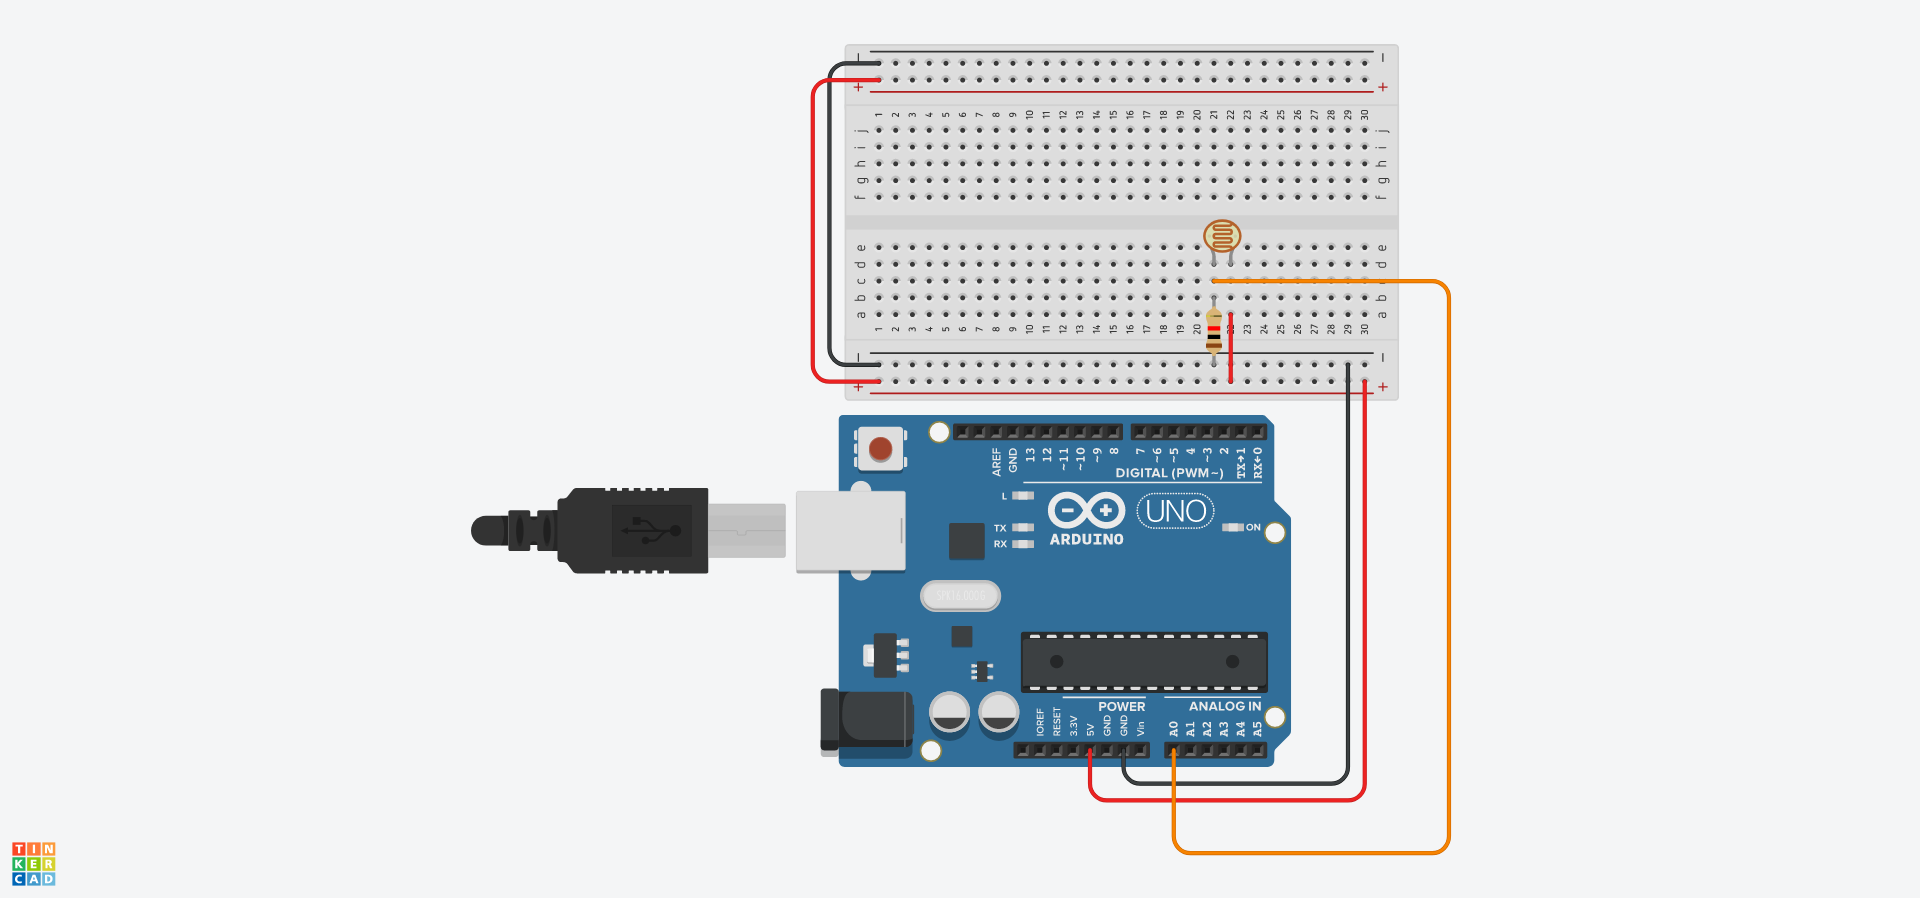
\includegraphics[width=0.9\textwidth]{images/p1_tkad.png} 
         \caption{Diagram of connections}
         \label{fig:connections1}
     \end{subfigure}  \hfill
    \caption{Circuit diagram and connection representation of Part IV (please note, these are obviously not related. This is an example of how to create a figure)}
    \label{fig:part1}
\end{figure}

%NOTE put a UML diagram and then do the algorithmic thinking part

\begin{algorithm}
\caption{Psuedocode for Part 1}\label{alg:part1}
\begin{algorithmic}[1]
\State REQUIRE a LightSensor object with an analog input pin
\State BEGIN the Serial on port 9600
\While{True}
\State READ the value from the analog input pin
\State PRINT the value read by from the analog input pin to the terminal.
\State DELAY 100ms
\EndWhile
\end{algorithmic}
\end{algorithm}

\subsection{Part II}\label{Part2Subsection}
Part 2 involved connecting two continuous servos to a 5V power supply and to GND, wired through a mini breadboard. Their rotation was controlled with a connection of the left servo to pin 13 and the right servo to pin 12. The code for this part was structured in the form of a Driver class, as depicted in the UML class digram of Figure~\ref{fig:uml2}. It was observed that writing the value of 1500 to the servos resulted in no movement, while values greater than 1500 led to clockwise rotation at faster speeds the higher the value, while those below 1500 resulting in faster anticlockwise rotation. The pseudocode has been omitted in favour of the functionality being explained in the UML diagram.

\begin{figure}[ht]
    \centering
      \begin{subfigure}[b]{0.2\textwidth}
         \centering
         \includegraphics[width=0.3\textwidth]{images/LED.png} 
         \caption{Circuit Diagram}
         \label{fig:Circuit_diagram2}
     \end{subfigure}
     \begin{subfigure}[b]{0.2\textwidth}
         \centering
         \includegraphics[width=0.9\textwidth]{images/lab_report_pic.png} 
         \caption{Diagram of connections}
         \label{fig:connections2}
     \end{subfigure}  \hfill
    \caption{Circuit diagram and connection representation of Part IV (please note, these are obviously not related. This is an example of how to create a figure)}
    \label{fig:part2}
\end{figure}


\subsection{Part III} \label{Part3Subsection}
Part 3 involved combining the functionality of continuous servos and light sensors to emulate how a maze navigating robot might behave. The circuit mostly uses the same layout as Part~\ref{Part2Subsection} with the addition of two light sensors connected to 5V power, a 10K Ohm resistor to GND and to analog input pins. Using the classes previously constructed in Figure~\ref{fig:uml1} and Figure~\ref{fig:uml2}
%(Example text of how to use subfigures). For this part, we were not provided a circuit diagram or design. Figure~\ref{fig:Circuit_diagram} shows our circuit diagram and Figure~\ref{fig:connections} shows a representation of how the components can be wired up to the Arduino.

\begin{figure}[ht]
    \centering
      \begin{subfigure}[b]{0.2\textwidth}
         \centering
         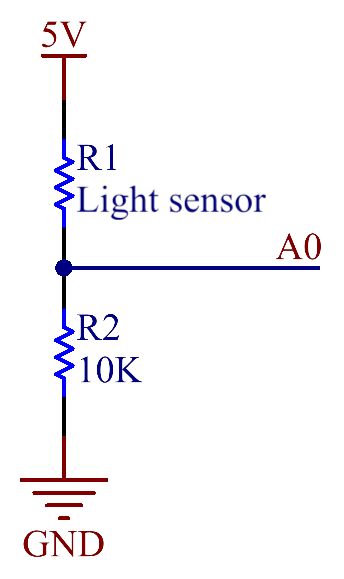
\includegraphics[width=0.2\textwidth]{images/pt1.png} 
         \caption{Circuit Diagram}
         \label{fig:Circuit_diagram3}
     \end{subfigure}
     \begin{subfigure}[b]{0.2\textwidth}
         \centering
         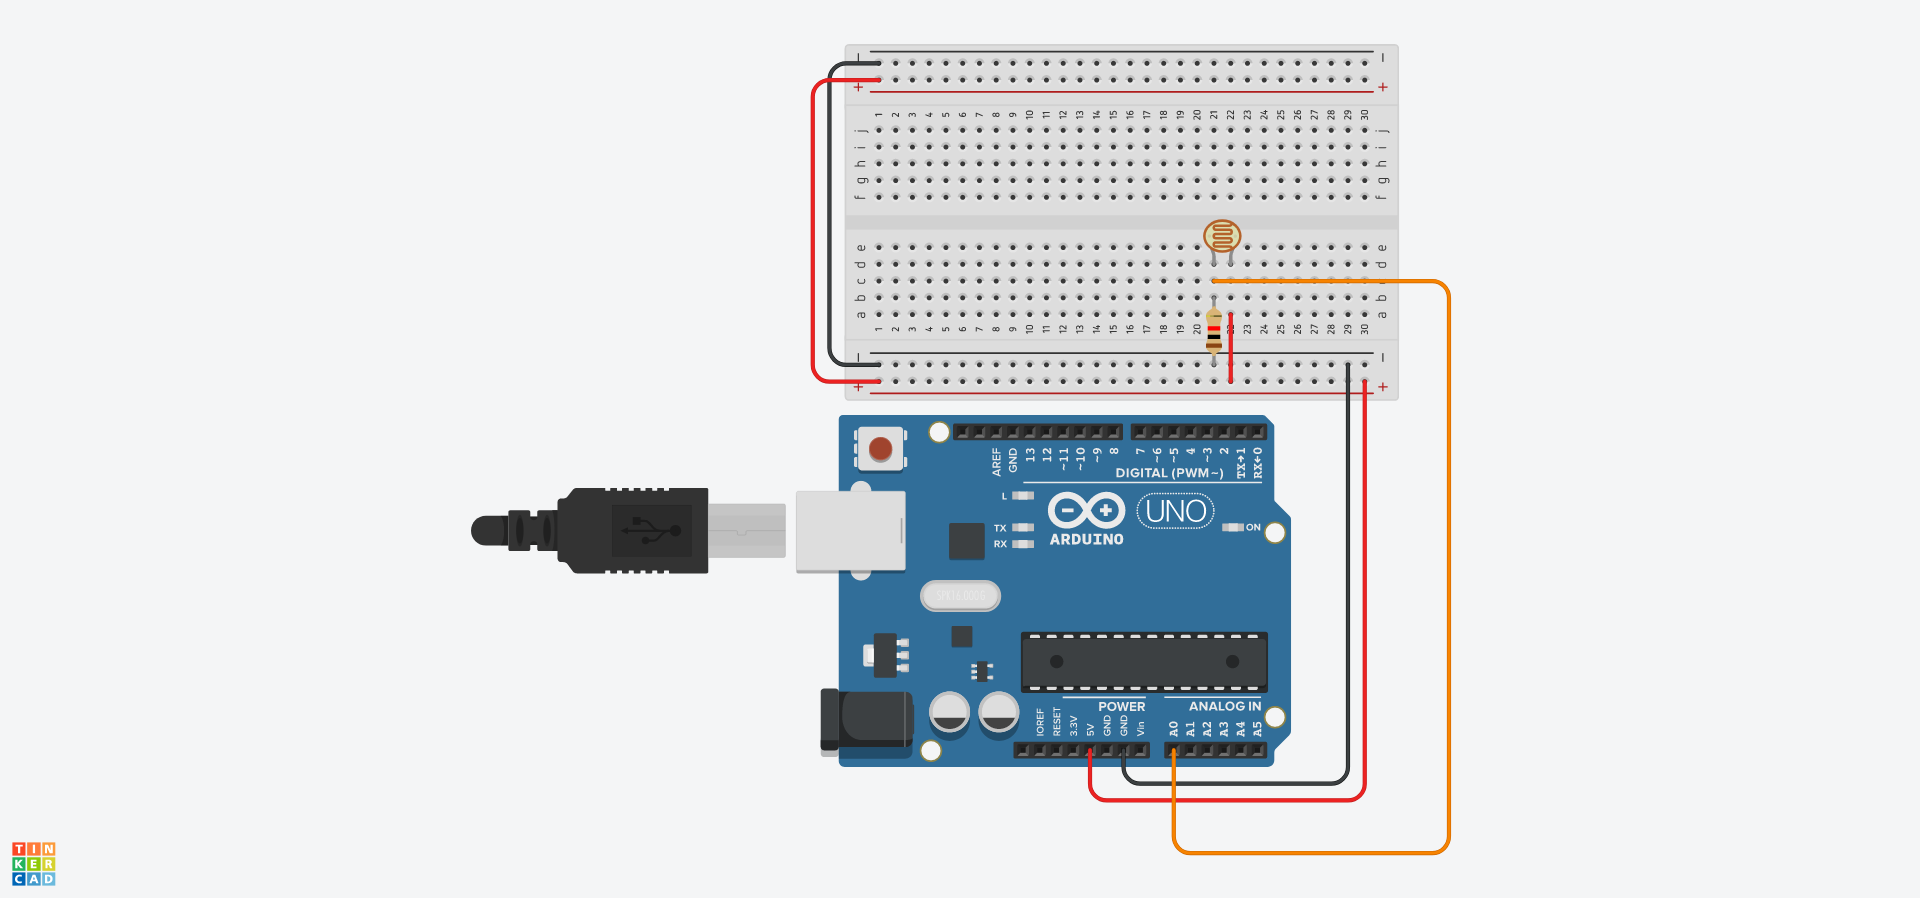
\includegraphics[width=0.9\textwidth]{images/p1_tkad.png} 
         \caption{Diagram of connections}
         \label{fig:connections3}
     \end{subfigure}  \hfill
    \caption{Circuit diagram and connection representation of Part IV (please note, these are obviously not related. This is an example of how to create a figure)}
    \label{fig:part3}
\end{figure}

%NOTE put a UML diagram and then do the algorithmic thinking part

\begin{algorithm}
\caption{Psuedocode for Part 1}\label{alg:part1}
\begin{algorithmic}[1]
\State CONSTANT mSpeedMag = 100
\State CONSTANT lSpeedMag = 50
\State REQUIRE 2 LightSensor objects connected to analog input pins
\State REQUIRE 1 Driver object with it's servos attached
\While{True}
    \State CALL forward() method of the Driver class WITH mSpeedMag
    \State DELAY 3000ms
\If{left Light Sensor's value is < 2V}
    \State CALL left() method of the Driver class WITH lSpeedMag
    \State DELAY 3000ms
\ElsIf{right Light Sensor's value is < 2V}
    \State CALL right() method of the Driver class WITH lSpeedMag
    \State DELAY 3000ms
\EndIf
\EndWhile
\end{algorithmic}
\end{algorithm}

\section{Results}
Describe the success/failure of your work.
Highlight any limitations! (this shows understanding)
% FINITE STATE MACHINE THINGY -- MAKE WITH MERMAID?

\section{Relation to real-world electronics}

The IR sensors can be used for night vision cameras. It is mentioned in \cite{elec1601_notes} that the wavelength of IR is used for remote control of electronics as as TVs. Extending from this real world application, the sensors used in the exercise could be used to control the maze navigating robot for the assignment. This can already be seen by remote controlled toy cars.

%Describe how what you learnt in this lab exists as part of a real devices/products you use, or as an alternative, describe a project you could invent based on what you have learnt.
For this section, you can move beyond an Arduino, but it should be based on  sensors/actuators related to the lab exercise.

%Example: a light sensor could be connected to alarm to remind you to put on sunscreen. However, try to elaborate here (e.g. it connects via wifi to your phone and creates a notification). 

\begin{itemize}
  \item {Discuss connections/sensors (suggest what is required to implement this - use drawings as necessary). This would involve fitting the robot with and IR receiver to respond to an IR emitter on a remote.}
  \item {Discuss pseudo code required to get it to work (this can be very high level (e.g. detect light level -> test against threshold -> send information via wifi to phone) 
  The code would involve: polling for an IR signal from the robot -> triggering an interrupt if triggered -> change in functionality, such as increasing or decreasing speed}
  \item {Discuss challenges, risks and difficulties to get it working/what could go wrong (e.g calibration for different environments)/fragility of components. Also discuss safety issues.
  The IR sensor would have to be exposed and visible from from the perspective of the emitter. This would pose a challenge if the maze}
\end{itemize}

\section{Conclusion}
Describe to what extent your stated learning outcomes were met and what you learnt.

\bibliographystyle{ieeetr}
\bibliography{references/ref}

\appendix

Any additional information. Please be aware, anything in this section may not be marked - it cannot contain anything critical. 

\end{document}


